\section{Waves from moving bodies}\label{sec:waves}

\begin{quote}
\textbf{In plain words.} Anything that is whirled, shaken or struck sends out
gravitational waves. But a wave cannot show detail smaller than its own
length, and these waves are longer than the thing that makes them by the same
factor that light is faster than the thing moves. A spinning flywheel is a
dot. The dot does carry a message: its polarization tells which way the wheel
is turning.
\end{quote}

Outside the near zone a source of mass quadrupole moment $Q_{ij}(t)$ produces
the strain
\begin{equation}\label{eq:quadrupole}
h_{ij}^{\TT}(t, r) = \frac{2G}{c^{4} r}\,
\ddot Q_{ij}^{\TT}\!\left(t - \frac{r}{c}\right),
\end{equation}
and radiates the power $P = (G/5c^{5})\,\langle \dddot Q_{ij}\,\dddot Q_{ij}
\rangle$. For two masses $m$ a distance $d$ apart, turning about their centre
at angular velocity $\Omega$,
\begin{equation}\label{eq:dumbbell}
P = \frac{8}{5}\,\frac{G m^{2} d^{4}\,\Omega^{6}}{c^{5}} .
\end{equation}
Two one-kilogram masses a metre apart, spun sixteen times a second, radiate
$4\times10^{-41}\,\mathrm{W}$: one graviton every fifteen years.

\paragraph{Every body is a point.} The waves of Eq.~\eqref{eq:dumbbell} have
twice the rotation frequency, so their wavelength is $\lambda = \pi c/\Omega$,
while the masses move at $v = \Omega d/2$. Hence
\begin{equation}\label{eq:unresolved}
\frac{\lambda}{d} = \frac{\pi}{2}\,\frac{c}{v} ,
\end{equation}
and the same holds, up to a factor of order one, for any body whose parts move
at speed $v$. The wavelength exceeds the body by the factor by which light
outruns it. No aperture can resolve an object smaller than the wavelength it
is seen by, so each moving body is a point in its own radiation.

\paragraph{What the point tells.} The radiation is not the same in all
directions, and it is polarized (Figure~\ref{fig:quadrupole}). Along the axis
of rotation it is strongest and circularly polarized, with the handedness of
the rotation; in the plane of rotation it is eight times weaker and linearly
polarized. From the polarization alone, a camera can read the axis and sense
of a rotor it cannot resolve.

\begin{figure}
\centering
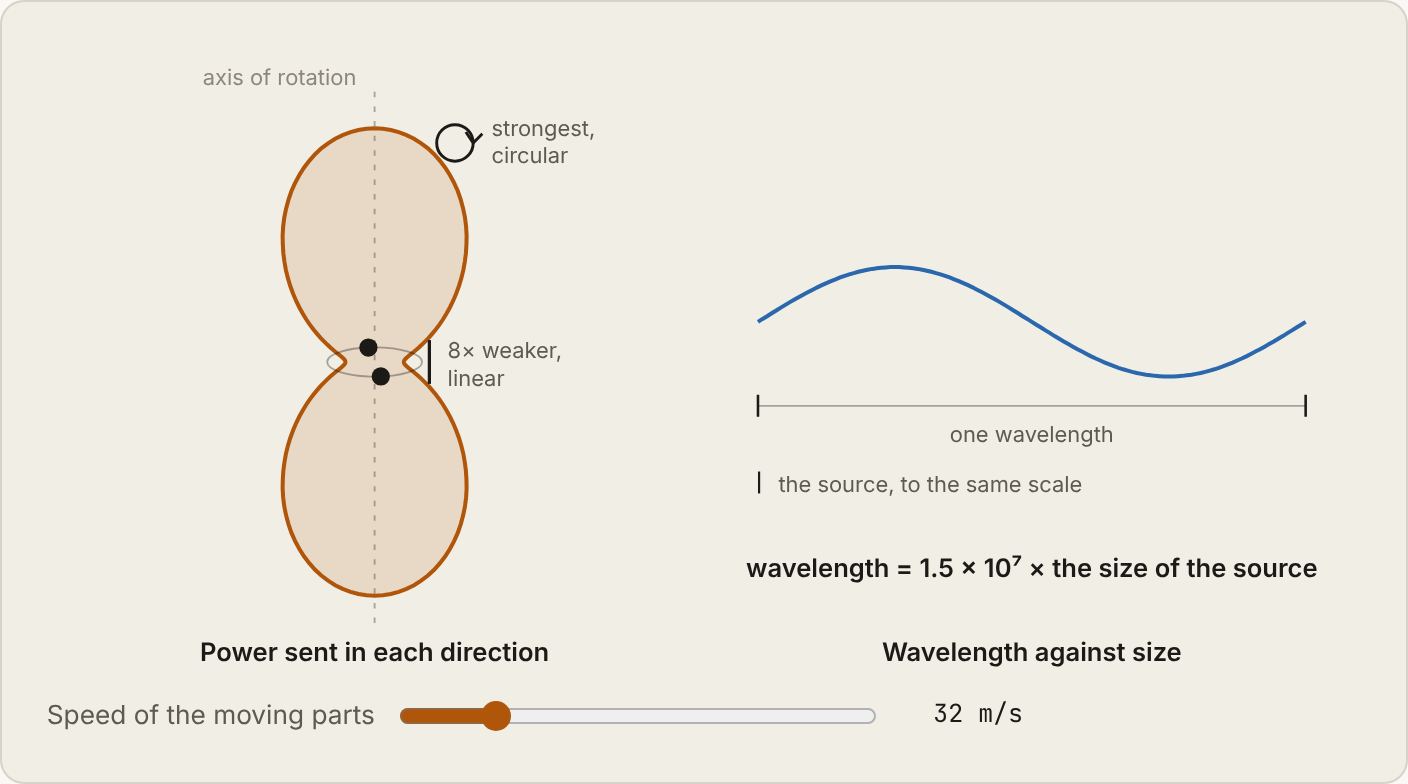
\includegraphics[width=\linewidth]{figures/quadrupole.png}
\caption{Radiation from a spinning pair of masses. Left: the power sent in
each direction, strongest along the axis of rotation. The small figures show
the polarization: circular along the axis, linear in the plane of rotation.
Right: the wavelength compared with the size of the source,
Eq.~\eqref{eq:unresolved}, for a chosen speed.}\label{fig:quadrupole}
\end{figure}

\paragraph{What does not radiate.} The source of the wave field is the part of
the stress that is transverse to the line of sight and has no trace. Steady
motion in a straight line has no changing quadrupole and radiates nothing. Nor
does anything that keeps spherical symmetry, however violently it pulsates.
And a pressure that is the same in all directions is pure trace: it is removed
exactly by the projection in Eq.~\eqref{eq:quadrupole}, a statement we have
verified numerically. The camera sees shear and lopsided motion, not pressure.

Because everyday speeds are so far below that of light, these effects cannot
be shown at human scale. The demonstrations that accompany this paper include
a clearly labelled mode in which the speed of light is lowered to walking
pace, so that the patterns of Figure~\ref{fig:quadrupole} become visible
around ordinary moving objects.
